\chapter{REVIEW OF METHODS FOR ELECTRICAL SOURCE RECONSTRUCTION}
\label{ch:review}
% \pagestyle{plain}

%textwidth in inches: \printinunitsof{in}\prntlen{\textwidth}

%At some point, cite \cite{grech2008review}.

The forward model discussed in Chapter \ref{ch:forward} can be summarized in the following matrix equation
\begin{equation*}
\Y = \G\, \ppar{ \SA + \nu } + \varepsilon
\label{eq:general}
\end{equation*}
where $\Y \in \R^{M\times T}$ encodes the EEG measurements over time, $\SA$ encodes the magnitudes of a finite set of distributed dipoles with known locations, and $\G \in \R^{M\times N}$ is a mixing operator referred to as the Leadfield matrix.

The terms $\nu \in \R^{N\times T}, \varepsilon\in\R^{M\times T}$ represent additive noise within the true values for the dipoles and sensors, respectively. 
%
Different authors have proposed different assumptions for such noise terms, some of which will be discussed later.

In chapter \ref{ch:forward}, it was discussed that if the orientation is known, then we can use $\SA\in \R^{N\times T}$, and otherwise, we should use $\SA\in \R^{3N\times T}$ from decomposing each dipole as the sum of dipoles with known orientations, parallel to the $x$-, $y$- and $z$-axis.
%
Since the cases of known and unknown dipole orientations don't significantly change the model formulation, they will be treated as a single model whenever possible.

Within the context of Electrical Source Reconstruction, the computation of the leadfield matrix is referred to as the Forward Problem.
%
This computation implies a large number of steps: identification of tissues from anatomical MRI or similar, construction of triangulated surfaces representing anatomical regions of interest (which may be simplified), setup of several PDEs within the anatomical regions as geometric domain, and the numerical solution of said equations by either BEM or FEM (or a different method).

All these points were discussed in Chapter \ref{ch:forward}. 
%
Thus, after this point, we will consider the leadfield matrix $\G$ to be given for each set of anatomical data and electrode montage.

\section{Inverse problem formulations}

The main aim of this work will be the task of `recovering' $\SA$ once the data $\Y$ and some additional assumptions are considered.

In the absence of biological noise ($\nu = 0$),
the most straightforward path of action is to find the $\SA$ that minimizes the reconstruction error
\begin{equation}
\hat{\SA}_{\text{naive}} =
\argmin_{\SA}\, \nnorm{\G\, \SA- \Y}_F^2 %+ \lambda\, f\ppar{\mathbf{S}}
\label{est:naive}
\end{equation}
with $\nnorm{A}_F$ the Frobenius norm of $A\in \R^{M\times N}$, defined as
\begin{equation}
\nnorm{A}_F =
\ppar{
\sum_{n=1}^N \sum_{m=1}^M \spar{A(m,n)}^2
}^{1/2}
\end{equation}

The expression in \eqref{est:naive} represents
an ill-posed problem due to (1) not having a unique solution and (2) changing significantly with small changes in the parameters.
%
The first statement is straightforward since we assumed $M\ll N$.
%
The second statement becomes clear if we choose the Least-Square solution,
\begin{equation}
\hat{\SA}_{\text{LS}} =
\G^T \ppar{\G\, \G^T}\pinv \Y
\end{equation}
where $A\pinv$ is the Moore-Penrose pseudoinverse of $A=\G\, \G\trans$.

It can be proven that the eigenvalues of $A\pinv$ are given by
\begin{equation}
\ppar{\sigma_i}\pinv =
\begin{cases}
\sigma_i\iinv, &\text{if } \sigma_i\neq 0 \\
0, &\text{otherwise}.
\end{cases}
\end{equation}
where $\sigma_i$ are the eigenvalues of $A=\G\, \G\trans$. 
%
Notice that the case $0\neq \sigma_i \approx 0$ leads to $\hat{\SA}_{\text{LS}}$ being `unstable' as a function of $\G$ and $\Y$.

As is discussed later, one way to alleviate the instability of the Least-Squares estimator is to modify the inverse problem by introducing a regularisation parameter $\lambda$, resulting in
\begin{equation}
\hat{\SA} = \argmin_{\SA}\, \nnorm{\G\, \SA - \Y} + \lambda\, f\ppar{\SA}
\label{est:gral}
\end{equation}
with $\lambda>0$ and $f: \R^{M\times T} \rightarrow \R_+$ a penalization function, usually related to the norm of $\SA$.
%
It will be shown how this formulation naturally results from certain assumptions, but it can also be designed to impose certain desirable properties on the solution.

\subsection{Minimal Norm Estimator}

For this estimator, we assume that both the sensor and internal noise are Gaussian random variables, independent in time and space, and with constant variance, i.e.
\begin{align}
\nu &\sim \norm\ppar{0, \sigma^2 \id_N \otimes \id_T  } \\
\varepsilon &\sim \norm\ppar{0, \lambda^2 \id_M \otimes \id_T}
\end{align}

The Maximum A Posteriori (MAP) estimator of $\SA$ is defined as
\begin{align}
\hat{\SA}_\text{MAP} 
&=
\argmax_\SA\,\, \prob\ppar{ \SA \given \Y }
\nonumber \\
&=
\argmax_\SA\,\, \prob\ppar{ \Y \given \SA }\, \prob{\SA}.
\end{align}

The above problem can be simplified by (1) taking the logarithm of the expression since $\log$ is a monotonic function, and by (2) considering the independence in time so that columns of $\SA$ are computed independently, and (3) considering the normal distribution of $\nu$ and $\varepsilon$.
%
Thus we have
\begin{align}
\hat{\SA}(:,t)_\text{MAP} 
&=
\argmax_\SA \,\, \log\ppar{ \prob\ppar{ \Y(:,t) \given \SA }\, \prob\ppar{\SA} }
\nonumber \\
&=
\argmax_\SA \,\,
- \frac{1}{2\sigma^2} \nnorm{\G\, \SA - \Y(:,t)}_2^2 
- \frac{1}{2\lambda^2} \nnorm{\SA }_2^2 
\nonumber \\
&=
\argmin_\SA \,\,
\nnorm{\G\, \SA - \Y(:,t)}_2^2 
+ \frac{\sigma^2}{2\lambda^2} \nnorm{\SA }_2^2 
\end{align}

Notice how the MAP estimator can be interpreted as a regularized optimization problem in the form of \eqref{est:gral}.
%
Since the MAP estimator is obtained by minimizing the norm of $\SA$ (in particular, the $\ell_2$ norm), it is referred to as the Minimal-Norm Estimator (MNE).
%
This designation is ambiguous since many other estimators depend on minimizing some norm of the sources; thus, `minimal-norm estimator' refers to a family of estimators. 
%
To avoid confusion, this particular estimator will be referred to simply as MNE in this work.

The MNE estimator admits a closed-form solution as follows,
\begin{equation}
\hat{\SA}_\text{MNE}
=
\hat{\SA}_\text{MAP}
=
\G\trans\ppar{ \G\, \G\trans + \frac{\sigma^2}{\lambda^2}\id_M }\iinv \Y
\end{equation}

\subsection{Weighted Minimal Norm Estimator}
\label{sec:wMNE}

This method incorporates the assumption that smaller coefficients in the leadfield matrix scale the contribution of deep dipoles located far from the scalp.
%
These deeper dipoles must have larger magnitudes to contribute similarly to shallow dipoles in the generation of EEG.
%
The overall effect is that deep dipoles are misrepresented in the MNE estimator and often deleted.
%
This assumption can be encoded by considering the following noise term,
\begin{align}
\nu &\sim
\norm\ppar{
0, 
W\iinv \otimes \id_T
}
\\
W &=
\text{diag}
\ppar{ \nnorm{\G(:,1)}_2, \nnorm{\G(:,2)}_2, \dots, \nnorm{\G(:,N)}_2 }
\label{det:wMNE}
\end{align}

In order to alleviate the effect mentioned above, the depth-weighting matrix $W$ is introduced.
%
The Weighted Minimal Norm Estimator (wMNE) is then defined as
\begin{align}
\hat{\SA}_\text{wMNE} 
&=
\ppar{\G\trans \G + \lambda\, W^T W}\pinv \G^T \Y \\
&=
\G\trans
\ppar{\G \ppar{W\trans W}\iinv \G\trans + \lambda\, \id_M}\pinv \Y
\label{est:wMNE}
\end{align}

\subsection{LORETA}

The Low-Resolution Electric Tomography (LORETA) estimator was proposed by Marqui\cite{sloreta}.
%
One key idea from this method is to use a Laplacian operator to impose spatial smoothness over $\SA$ and use the same depth-weighting from wMNE.

In its original formulation, the dipoles are assumed to be located on a cubic grid with a distance $d$ between neighboring dipoles. 

The LORETA estimator can be expressed as an optimization problem
\begin{align}
\hat{\SA}_\text{sLORETA} 
&=
\argmin_\SA \,
\nnorm{ B\, W\, \SA } _F^2 
\nonumber \\
&\text{s.t. }
\G\, \SA = \Y
\end{align}
with $W$ as in \eqref{det:wMNE}, and $B$ the laplacian operator defined as
\begin{equation}
B(n_i, n_j) =
\begin{cases}
6/d^2, &\text{if } n_i=n_j \\
-1/d^2, &\text{if } \nnorm{\rr_{n_i}-\rr_{n_j}}_2 = d \\
0, &\text{otherwise}
\end{cases}
\end{equation}
where $d$ is the distance between dipoles. On a cubic grid, exactly 6 dipoles satisfy the second condition when the $n_i$-th dipole is far from the cortex.

The estimator is computed as follows:
\begin{equation}
\hat{\SA}_\text{LORETA} 
= 
\ppar{ W\, B\trans\, B\, W }\iinv
\G\trans
\spar{ \G \ppar{ W\, B\trans\, B\, W }\iinv \G\trans }\pinv
\Y
\label{est:LORETA}
\end{equation}

\subsection{sLORETA}

The standardized Low-Resolution Electric Tomography (sLORETA) estimator was proposed by Marqui \cite{sloreta}.
%
Despite their similar name, LORETA and sLORETA are two different methods.
%
The sLORETA estimator considers the following minimization problem
\begin{equation}
\hat{\SA}_\text{sLORETA} 
= 
\argmin_{\SA}\, \nnorm{\G\, \SA - \Y - c \ones }_F^2 + \lambda\, \nnorm{\SA}_F^2
\end{equation}
with $\ones=\{1\}^{M\times 1}$ a column vector of ones.

The underlying assumption is that the measurements are re-referenced to the average, i.e., the raw observations $\Y_0\in \R^{M\times T}$ are pre-processed as follows
\begin{equation}
\Y = \ppar{ \id_M - H } \Y_0
\end{equation}
with $H \in \R^{M \times M}$ an averaging operator constructed as
\begin{equation}
H = \ppar{\ones_M \ones_M\trans}/\ppar{\ones_M\trans \ones_M}.
\end{equation}

Alternatively, we can construct $H$ element-wise as
\begin{equation}
    H(m_1, m_2) = \frac{1}{M}
\end{equation}
for $m_i = 1, 2, \dots, M$ and $i=1,2$.

It is relevant to mention that this type of re-reference can be interpreted as constructing a phantom electrode with neutral electric activity and using it to close the recording circuit.
%
This process is expected to eliminate noises that are common to all electrodes.

Assuming that $\Y$ was re-referenced to the average, then the parameter $c$ is always zero, and the estimator is as follows
\begin{equation}
\hat{\SA}_{\text{sLORETA}} =
\G^T H 
\ppar{
H\, \G \,\G\trans 
H + 
\lambda H
}\pinv
\Y
\label{est:sLORETA}
\end{equation}

\subsection{Multivariate Source Prelocalization (MSP)}

The MSP estimator proposed by Mattout \cite{mattout2005multivariate} incorporates the idea of using Single Value Decomposition (SVD) to produce a subspace that captures the most relevant information in $\Y$ and $\G$, then gets the sources more correlated with their projections into that space.
%
The obtained information is later used to construct a weight matrix, so the final estimation is similar to wMNE.
\begin{equation}
\hat{\SA}_\text{MSP} = \argmin_{\SA} \nnorm{\Y - \G \SA}_F^2 + \lambda\nnorm{W_\text{MSP} \SA}_F^2
\end{equation}

The leadfield matrix is column-normalized as in \ref{det:wMNE}, and the SVD decomposition is performed, 
\begin{align}
\Gbar &=  \G\, W_G\iinv = \U \mathbf{\Lambda} \V\trans
\\
W_G &= 
\text{diag}
\ppar{ \nnorm{\G(:,1)}_2, \nnorm{\G(:,2)}_2, \dots, \nnorm{\G(:,N)}_2 }
\end{align}
with $\U\in \R^{M\times M},\V\in \R^{N\times N}$ such that $\U\trans \U = \id_M, \V\trans\V = \id_N$, and $\mathbf{\Lambda} \in \R^{M\times N}$ a matrix with the singular values of $\Gbar$ in descending order on its diagonal.

The first $s$ columns of $\U$ are selected based on the Velicer criterion \cite{velicer1996criterion},
\begin{align}
\U_s 
&= 
\spar{ \U(:,1), \U(:,2), \dots, \U(:,s) }
\end{align}

$\Y$ is normalized on a similar way as $\Gbar$, and then it is projected into $\U_s\, \U_s\trans$,
\begin{align}
\Ybar_s 
&=
\U_s \U_s^T \Ybar = \U_s \U_s^T W_Y \Y
\\
W_Y &= \diag{ \nnorm{Y(:,1)}_2, \nnorm{Y(:,2)}_2, \dots, \nnorm{Y(:,T)}_2 }
\\
\mathbf{A}_s &= \ppar{\Gbar\trans \Ybar_s}\, \ppar{\Gbar\trans \Ybar_s}\trans
\end{align}

The authors of MSP propose interpreting $\mathbf{A}_s$ as a correlation matrix of the sources within the resulting space.
%
Following this interpretation, the authors define {Activation Probability Map} (APM) as
\begin{align}
{D}_s(j) = \mathbf{A}_s(j,j) = \nnorm{\Gbar(:,j)\trans \Ybar_s  }_2^2
\end{align}
%with the additional information that ${D}_s(j) \sim Gamma(a,b)$.

The MSP weigh matrix, $W_\text{MSP}$, is constructed as
\begin{equation}
W_\text{MSP}(j,j) = 1-{D}_s(j)
\end{equation}
leaving the MSP estimator as follows,
\begin{align}
\hat{\SA}_\text{MSP} &=
\spar{W_\text{MSP}}^{-2} \G^T \ppar{ \G\spar{W_\text{MSP}}^{-2}\G^T + \lambda \id_m  }^{-1} \Y
\label{est:MSP}
\end{align}

\begin{comment}
\subsection{Minimum Current Estimate (MCE)}

Proposed by Uutel, H\"{a}m\"{a}l\"{a}inen, Somerselo.
%
This estimator incorporates the assumption that the source patches are `sparse', i.e., most of the dipoles have a magnitude of zero.

Minimizing the number of non-zero entries of $\SA$ can be achieved by minimizing $\nnorm{\SA}_{1,1}$, which is defined as
\begin{equation}
\nnorm{A}_{1,1} = \sum_{m=1}^M \sum_{n=1}^N \abss{A(m,n)}
\end{equation}

The MCE estimator is defined as
\begin{align}
\hat{\SA}_\text{MCE} &=
\argmin_{\SA}\, \nnorm{\G\, \SA - \Y }_2^2 + \lambda\, \nnorm{\SA}_{1,1}
\label{est:MCE}
\end{align}

Unlike the other estimators described until this point, the MCE estimator does not admit a closed-form solution.
%
It can be solved efficiently using the Alternating Direction Method of Multipliers (ADMM) proposed by Boyd \cite{boyd2011admm}.

A thorough description of the ADMM methodology is beyond the scope of this chapter, and the interested reader should refer to the book by Boyd \cite{boyd2011admm}.
%
These algorithms are included to compare the results.
\end{comment}

\subsection{Mixed Norm Estimate (MxNE)}

This algorithm, proposed by Gramfort \cite{gramfort2012mixed}, incorporates the assumption that the source patches are sparse in space and smooth in time.
%Gramfort, M. Kowalski, and M. Hämäläinen, "Mixed-norm estimates for the M/EEG inverse problem using accelerated gradient methods," Phys Med Biol., vol. 57, no. 7, pp. 1937–1961, 2012.
%
This assumption is enforced by solving the following optimization problem.
\begin{align}
\hat{\SA}_\text{MxNE} &=
\argmin_{\SA}\, \nnorm{\G\, \SA - \Y }_F^2 + \lambda\, \nnorm{\SA}_{2,1}
\label{est:MxNE}
\end{align}
with $\nnorm{\SA}_{2,1}$ the $\ell_{2,1}$ norm of $\SA$.
%
In general, the bi-level $\ell_{p,q}$ norm is defined as
\begin{equation}
\nnorm{A}_{p,q} =
\ppar{\sum_{m=1}^M \ppar{ \sum_{n=1}^N \abss{A(m,n)}^p }^{q/p}}^{1/q}
\end{equation}

The MxNE estimator does not admit a closed-form solution but can be computed using the Alternating Direction Method of Multipliers (ADMM) or similar algorithms.
%
A thorough description of ADMM is beyond the scope of this chapter, and the interested reader should refer to the book by Boyd \cite{boyd2011admm}.

\begin{comment}
\subsection{SISSY}

The algorithm called Source Imaging based on Structured Sparsity (SISSY) was proposed by Becker ().
\end{comment}


%%%%%%%%%%%%%%%%%%%%%%%%%%%%%%%%%%%%%%%%%%%%%%%%%%%%%%%%
%%%%%%%%%%%%%%%%%%%%%%%%%%%%%%%%%%%%%%%%%%%%%%%%%%%%%%%%

\section{Methods for parameter selection}

From all the estimation methods described in the previous section, all of them converge in a general form
\begin{equation}
\hat{\SA}_\Theta = F\ppar{ \Y, \G; \Theta }
\end{equation}
with $\Theta$ a set of parameters that must be selected beforehand.
%
One particular case, referred to as linear estimator, occurs when the estimator can be written as
\begin{equation}
\hat{\SA}_\Theta
=
\mathbf{K}_{\Theta}\, \Y
\end{equation}
with $\mathbf{K}_{\Theta} \in \R^{N\times N}$ referred to as the Wiener kernel, or inversion kernel, which is approximately a right inverse of $\G$.
%
The collection of liner methods includes wMNE, FOCUSS, LORETA and their derivates, and MSP, among others. 

On the other hand, methods like MCE, MxNE, SiSSY, etc, are not linear and can't be assigned to a Wiener kernel.

This section reviews some heuristics for selecting the parameter set $\Theta$.
%
The wMNE estimator is a reference model since it depends on a single parameter.
%
However, the heuristics can be generalized to select multiple parameters by finding the minima/maxima of functions of multiple variables.
%
Such a generalization is not made explicit.

\subsection{L-curve}

This heuristic incorporates the idea that the parameter $\lambda$ balances the factors $\nnorm{\SA}_F^2$ and $\nnorm{\G\, \SA - \Y}_F^2$, trying to minimize both of them evenly \cite{Lcurve}.
%
To do that, define the quantities
\begin{align}
\rho(\lambda)
&=
\nnorm{\G\, \hat{\SA}_\lambda - \Y}_F^2
%=
%\nnorm{\G\, K_\lambda\Y - \Y}_F^2
\\
\eta(\lambda)
&=
\nnorm{\hat{\SA}_\lambda}_F^2 
%= 
%\nnorm{ K_\lambda \Y }_F^2
\label{det:Lcurve}
\end{align}

The L-curve denominations come from the graph of the parametric curve $\ppar{\rho(\lambda), \eta(\lambda) }$, which resembles the letter `L' in some cases.
%
This graph is typically displayed in log-log scale, i.e., the parametric curve $\ppar{\log\ppar{\rho(\lambda)}, \log\ppar{\eta(\lambda)} }$.
%
%stand from a log-log plot of the parametric curve $\ppar{\rho(\lambda), \eta(\lambda) }$, which has a characteristic appearance.

According to this criterion, the optimal value for $\lambda$ is the one on the point of maximal curvature of the parametric curve, often referred to as the `elbow' of the curve.
%
Look at the figure \ref{fig:tuning} for visual reference.

It is important to mention that the selection of parameters using the L-curve criterion depends on visual perception, and it may be affected by the precision with which the curve is constructed.
%
Without prior knowledge, $\eta$ and $\rho$ shall be computed for several potential values of $\lambda$.
%
Exploring the obtained parametric curve visually allows us to identify better the range where the optimal values may be found.

%The heuristic from this method is to select the value of $\lambda$ that leads to the closest point to the curving point in the plotted curve.

%Notice that the quantities $\eta, \rho$ can be computed relatively quickly for a small set of potential values of $\lambda$, and more points can be added to get a more precise curve.

%Notice that the parametric curve in \eqref{det:Lcurve} can be easily generalized for other quantities.

\subsection{Generalized Cross-Validation}

This heuristic is based on the principle of leave-one-out cross-validation and some approximations that make it computationally efficient. 
%
Although this method was proposed by Golub in 1979 \cite{GCV_Golub}, it remains popular for methods that admit an inversion kernel.

Following the leave-one-out principle, we consider $\Y^{[m]}\in\R{(M-1)\times T}$ and $\G^{[m]} \in \R^{(M-1)\times N}$ with the $m$-th sensor missing,
\begin{align}
\Y^{[m]} &=
\begin{bmatrix}
\Y(1,:) \\
\vdots \\
\Y(m-1,:) \\
\Y(m+1,:) \\
\vdots \\
\Y(M,:) 
\end{bmatrix},
\quad
\G^{[m]} =
\begin{bmatrix}
\G(1,:) \\
\vdots \\
\G(m-1,:) \\
\G(m+1,:) \\
\vdots \\
\G(M,:) 
\end{bmatrix}
\end{align}

Based on this incomplete information, we construct a restricted Wiener kernel, $K_\lambda^{[m]} \in \R^{N\times(M-1)}$, and a restricted estimation, $\SA_\lambda^{[m]} \in \R^{N\times T}$,
\begin{align}
K_\lambda^{[m]}
&=
\ppar{\G^{[m]}}\trans\ppar{ \G^{[m]}\, \ppar{\G^{[m]}}\trans + \lambda\id_M }\iinv
\\
\SA_\lambda^{[m]}
&=
K_\lambda^{[m]}\, \Y_\lambda^{[m]}
\end{align}

The cross-validation is incorporated by estimating the measurements from the $m$-th with information from $\SA_\lambda^{[m]}$ and then comparing it with the actual measurements.
%
By performing this procedure over all the sensors and averaging, we obtain the following quantity
\begin{equation}
V(\lambda) = 
\frac{1}{M}
\sum_{m=1}^M
\nnorm{ \spar{ \G \SA_\lambda^{[m]} }(m, :) - \Y(m,:) }_F^2
\label{det:GCV_pre}
\end{equation}

This quantity is approximated by the following
\begin{equation}
\text{GCV}(\lambda) = 
\frac{M\, \nnorm{\ppar{\G\, K_\lambda -\id_M }\, \Y}_F^2}{\text{trace}^2\ppar{\G\, K_\lambda - \id_M}}
\label{det:GCV}
\end{equation}

Although the definition of GCV is based on the leave-one-out cross-validation illustrated in equation \eqref{det:GCV_pre}, it is the expression on \eqref{det:GCV} the operative definition of GCV.
%
The latter expression represents a balance between $K_\lambda$ as a pseudo-inverse of $\G$ in general vs only for the current sensor data.

According to this criterion, the optimal value for $\lambda$ is the one that minimizes the function in \eqref{det:GCV}.
%, which can be extended easily to multiple parameters.
In other words,
\begin{equation}
    \lambda^\star_\text{GCV} = 
    \argmin_\lambda\,\, \text{GCV}(\lambda)
\end{equation}

It is important to emphasize that the approximation for the GCV error in equation \eqref{det:GCV} can only be computed for linear methods; for instance, estimators based on the $\ell_1$ norm or neural networks can't be tuned using GCV.

\subsection{Composite Residual and Smoothing Operator (CRESO)}

This heuristic incorporates the idea that the residual, $\nnorm{\G\, \SA - \Y}_F^2$, and the norm of the solution, $\SA_F^2$, should be approximately equal \cite{creso}.
%
To achieve that, the residual and norm are written as the following function, 
%referred to as the Composite Residual and Smoothing Operator (CRESO),
\begin{align}
    C\ppar{\lambda} &= 
\frac{d}{d\lambda} \spar{ -\nnorm{\G\SA_\lambda - \Y}_2^2 + \lambda \nnorm{\SA_\lambda}_2^2}
\nonumber \\
&=
\frac{d}{d\lambda} \spar{ - \nnorm{\ppar{\G K_\lambda + \id_M}\Y}_2^2 - \lambda \nnorm{K_\lambda \Y}_2^2}
\end{align}
with $K_\lambda \Y$ the inversion kernel, understood explicitly as a function of $\lambda$. 
%
This function is called the Composite Residual and Smoothing Operator (CRESO).

According to this criterion, the optimal value for $\lambda$ is the smallest solution to the equation $C(\lambda)=0$, or in other words,
\begin{equation}
    \lambda^\star_\text{CRESO} = 
    \min_\lambda \sset{\lambda\in \R_+ \given C(\lambda)=0}.
\end{equation}

\subsection{U-curve}

This heuristic incorporates the idea that both the largest among the residual and the solution's norm should be small; this is achieved by minimizing their reciprocals \cite{Ucurve}.
%
In particular, the following function is constructed
\begin{equation}
U(\lambda) = 
\nnorm{\G\SA_\lambda - \Y}_2^{-2} + \nnorm{\SA_\lambda}_2^{-2}
\end{equation}

Similar to the L-curve heuristic, the U-curve heuristic gets its denomination from the typical shape of the plot of $U(\lambda)$.

According to this criterion, the optimal value for $\lambda$ is the global minimum of $U(\lambda)$.
%
In other words,
\begin{equation}
    \lambda^\star_\text{U-curve} = 
    \argmin_\lambda\,\, U(\lambda)
\end{equation}

\begin{figure}
\centering
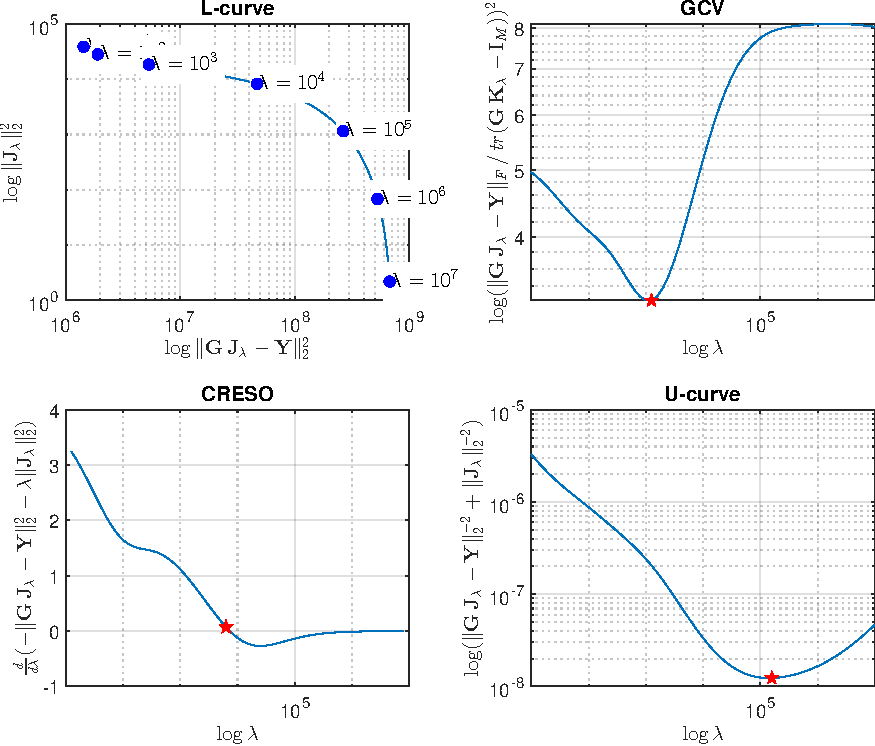
\includegraphics[width=1\linewidth]{./img_MATLAB/ParTuning_sLORETA}
\caption{Selection of parameters using various criteria: L-curve, Generalized Cross-Validation (GCV), Composite Residual and Smoothing Operator (CRESO), and U-curve. 
%
Each criterion's quantity of interest is computed for many candidate values of $\lambda$, then the optimal value is decided.
%
Data for these graphs was obtained from a single trial of synthetic data described in Chapter \ref{ch:numeric}. Data $\Y$ is constructed with no-noise, inversion kernel $\mathbf{K}_\lambda$ and the source estimate $\SA_\lambda = \mathbf{K}_\lambda \Y$ are computed using sLORETA
}
\label{fig:tuning}
\end{figure}

%%%%%%%%%%%%%%%%%%%%%%%%%%%%%%%%%%%%%%%%%%%%%%%%%%%%%%%%
%%%%%%%%%%%%%%%%%%%%%%%%%%%%%%%%%%%%%%%%%%%%%%%%%%%%%%%%

\section{Performance metrics}

\subsection{Definitions of a Source Patch Location}

In many early works, like the original paper for sLORETA \cite{sloreta}, synthetic data for ESI methods used `point sources' in the form of
\begin{equation}
    \SA_\text{ref}(n) = \begin{cases}
        1, &\text{if } n = n^* \\
        0, &\text{otherwise}
    \end{cases}
\end{equation}
with $n^*$ the index of one dipole.
%
Point sources are easy to evaluate in the forward model: we only need to select a column of $\G$ instead of performing a multiplication.

The location of a point source indexed by $n^*$ is $\rr_{n^*}$, a very straightforward definition.
%
On the other hand, there is no single unified definition for more complicated source distributions, including multiple source patches.

%There is no single definition for the location of the source in the case of multiple extended sources.
%
%In synthetic data with protocols similar to those of the next section, we use the `seed' node as the center of each source patch.
%
%It is also possible to use the dipoles with a maximal magnitude or the centers of mass with respect to the dipole magnitude.
%
%Since the minimal-norm estimators often produce many dipoles with small magnitudes, some authors use only dipoles whose magnitude is relatively large or which are close to the dipole with maximal magnitude.

%In this work, we employ an operative definition based on the latter.
%
%First, we estimate a patch $\mathcal{I}_i$ as the dipoles that are close to the $i$-th local maximum, indexed by $x_i$, and whose magnitude is significant enough to be relevant.
%\begin{align}
%x_i &= \argmax_{n} \nnorm{\SA_n}_2
%\nonumber \\
%&\phantom{=} \text{s.t. }
%n\not\in \mathcal{I}_j, j<i
%\\
%\mathcal{I}_i
%&=
%\sset{ n\in \sset{1, \dots, N} \given 
%\nnorm{r_n - r_{x_i}} < \nnorm{r_n - r_{x_j}} \text{ for } j<i,
%\nnorm{\SA_n}_2\geq \alpha\nnorm{\SA_{x_i}}_2 }
%\end{align}
%with $0<\alpha<1$; usually $\alpha=10\%$.

%With this information, the center of the patch is merely the center of mass with respect to $\nnorm{\SA}_2^2$,
%\begin{align}
%k_i = 
%\frac{\sum_{n\in \mathcal{I}_i} r_n \nnorm{\SA_n}_2^2 }{\sum_{n\in %\mathcal{I}_i} \nnorm{\SA_n}_2^2}
%\label{def:center1}
%\end{align}

%If the number of source patches is unknown, the patches can be identified sequentially by finding the local maximum of the dipoles not included in any patch; this process is repeated until all the dipoles with significant magnitude are classified.

%The operative definition in \eqref{def:center1} is consistent with the cited definitions for source location on synthetic source patched, even in the case of point sources.
%
%Thus, it can be used to determine the `true' centers of the source patches, $k_i$.
%
%However, the definition may deviate in the case of reconstructed sources.

%In this work, for the sake of comparability,
%
%%For evaluation purposes, 
%we employ the definition proposed by H\ "{a}m\" {a}l\" {a}inen []; this definition considers one single measurement in time and multiple disconnected source patches, each one created from a `seed dipole'. 
%
%Informally, a seed dipole is a dipole around which the source patch is constructed.

In this work, the location of a source patch, either the estimation or the reference, is defined as the center of mass with respect to magnitude.
%
%The reasoning for this decision is discussed in the following subsection.
%
This particular definition can be traced back to the paper by Molins et al. \cite{molins2008quantification}, and the reasoning for its use is discussed in the following subsection.

In order to establish a formal definition, we first must consider the concept of a seed dipole.
%
Informally, the idea of a seed dipole is that the source patch is constructed around it, and thus, the seed dipole is a proto-center for the source patch.
%
This definition only works for sources with known locations; thus, it is unusable for estimated sources.

One key property of a seed dipole, which will be later exploited, is that it must be one of the most active dipoles in the patch, i.e.
\begin{equation}
    \nnorm{\SA\ppar{k_p^*}} = \max\, 
    \sset{ \nnorm{\SA\ppar{n}} \given n\in \mathcal{I}_p }
\end{equation}

In the case of estimated sources, the role of seed dipoles can be fulfilled by local maxima of the estimated magnitudes.

Let be $k_1^*, k_2^*, \dots, k_{P} \in \sset{1, 2, \dots, N}$ the indexes of the seed dipoles.
%
Formally, the $p$-th source patch, $\mathcal{I}_p$, is defined as the set of dipoles that have significant activity and are closer to the $p$-th seed dipole, $k_p^*$ than to the other seed dipoles.
%
%In other words,
\begin{equation}
    \mathcal{I}_p = 
    \sset{n 
    \given
    \nnorm{\rr_n-\rr_{k_p^*}}_2 < \nnorm{\rr_n-\rr_{k_j^*}}_2
    \text{ for } p\neq j,
    \,\,
    \nnorm{\SA(n)}_2 \geq 
    \alpha \nnorm{\SA \ppar{k_p^*}}_2
    }
\end{equation}
where $\alpha\in [0,1]$ filters sources whose magnitude is very small;
%
for instance, we may set $\alpha = 10\%$ as a cutoff for significance.

In the case of estimated dipoles, the number of source patches can be adjusted algorithmically by joining or breaking other source patches.

The location of the $p$-th source patch, $\mm_p$, is defined as the center of mass of the dipoles in the source patch with respect to their magnitude,
\begin{equation}
    \mm_p = 
\frac{\displaystyle \sum_{n\in \mathcal{I}_p} \nnorm{{\SA}(n)}_2^2 \rr_n }{\displaystyle \sum_{n\in \mathcal{I}_p} \nnorm{{\SA}(n)}_2^2}
\end{equation}

Notice that this definition depends heavily on knowing the true locations of the seed dipoles, if any, so it can't be used with real data.

On the other side, the definition is trivially extended to the location of an estimated source patch,
\begin{equation}
    \hat{\mm}_p = 
\frac{\displaystyle \sum_{n\in \mathcal{I}_p} \nnorm{\hat{\SA}(n)}_2^2 \rr_n }{\displaystyle \sum_{n\in \mathcal{I}_p} \nnorm{\hat{\SA}(n)}_2^2}
\end{equation}

This definition is deficient when an ESI method does not recover all source patches, in which case the performance is overestimated.

\subsubsection{Other Definitions}

Although the definition presented is compatible with other definitions in the case of a single source patch, it is not the only one.

For instance, some authors have used the location of the seed dipole as the location of the source patch
\begin{equation}
    {\mm}_p = \rr_{k_p^*}
\end{equation}
which shouldn't be very different from the center of mass if the source patch is symmetric and centered around the seed.
%
For example, these assumptions are broken for volumetric source patches near the cortex.

Some authors define the location as the local maximum magnitude
\begin{equation}
    {\mm}_p = \sset{\rr_k \given k = \argmax_n\,\,
    \sset{\nnorm{\SA(n)} \given n\in \mathcal{I}_p }
    }
\end{equation}
which is also very similar if the source patch is symmetrical and decays monotonically far from the seed.
%
This is not the case if $\nnorm{\SA(n)}$ is constant in the patch.

The source location based on maximal magnitude can be trivially extended to define the location of an estimated source patch
\begin{equation}
    \hat{\mm}_p = \sset{\rr_k \given k = \argmax_n\,\,
    \sset{\nnorm{\hat{\SA}(n)} \given n\in \mathcal{I}_p }
    }
\end{equation}

This definition is not robust to noise if the true source is large in space.

\subsection{Distance Localization Error (DLE)}

Given the definitions of the true and estimated centers for the source patches, the Distance Localization Error is defined as
\begin{equation}
\text{DLE} = 
\frac{1}{P} \sum_{p=1}^P \nnorm{ \mm_p - \hat{\mm}_p }_2
\label{def:DLE}
\end{equation}
with $P$ the number of true source patches.
%
This definition does not account for whether the reconstruction has more or fewer source patches than it should.

\subsection{Spatial Dispersion (SD)}

This metric, proposed by Molins et al \cite{molins2008quantification}, is defined as
\begin{equation}
\text{SD}
=
\ppar{
\frac{ \displaystyle
\sum_{p=1}^P \sum_{n\in \mathcal{I}_p} \nnorm{\hat{\SA}(n)}_2^2\, \nnorm{\rr_n-\mm_p} }{\sum_{n=1}^N \nnorm{\hat{\SA}(n))}_2^2}
}^{1/2}
\end{equation}

This quantity can be understood as a variance in space for the source location. 
%
A small spatial dispersion is desirable.

It is possible to replace $\hat{\SA}$ for ${\SA}$ in order to compute a `baseline' spatial dispersion for source patches, which is especially useful if they are large in space.

\subsection{Relative Mean Square Error (rMSE)}

Also referred to as relative Reconstruction Error, this metric represents the estimation error for the dipole magnitudes. 
%
It is defined as
\begin{equation}
\text{rMSE} = 
\frac{\nnorm{\SA - \hat{\SA}}_2}{\nnorm{\SA}_2}
\end{equation}

\begin{comment}
\subsection{Effective Mean Square Error (fMSE)}

This metric is similar to the rMSE, but as perceived by the sensors.
%
It is defined as
\begin{equation}
\text{fMSE} = 
\frac{\nnorm{\G\ppar{\SA - \hat{\SA}}}_2}{\nnorm{\G\, \SA}_2}
\end{equation}
\end{comment}

\subsection{Area Under Receiver-Operator Curve (AUROC)}

It is possible to interpret the estimation from Electric Source Imaging as a binary classification problem over the dipoles; this is done by considering active/non-active classes.
%
This interpretation is consistent with the usability of ESI data to identify brain regions that are `active' during specific cognitive or pathological processes.

%Within this interpretation, the active/non-active labels can be created in many ways. 
%
%H\"{a}m\"{a}l\"{a}inen proposed using the relative magnitude to 
%\begin{align}
%\mathcal{A}^{\text{ref}}(\beta)
%&=
%\sset{n\in\sset{1, \dots, N} \given  }
%\end{align}

%This metric, very common in Data Science, is used in this context by interpreting the dipoles' magnitude as scores to label them as active or non-active.
%
A natural assumption in this context, already discussed in Chapter \ref{ch:forward}, is that dipoles with large magnitude are related to brain regions displaying coherent activity.

We consider the target labels as reference, ${\mathcal{R}: [0,1] \rightarrow \sset{0,1}^N}$ and the inferred labels as estimations, $\mathcal{E}: [0,1] \rightarrow \sset{0,1}^N$.
%
The assumption of active dipoles/regions is modeled by constructing the labels as follows,
\begin{align}
\mathcal{R}_\beta(n)
&=
\begin{cases}
1, &\text{if }
\nnorm{\SA(n)}_2 \geq \beta \max_{n'}\sset{\nnorm{\SA(n')}_2}
\\
0, &\text{otherwise}
\end{cases}
\\
\mathcal{E}_\beta(n)
&=
\begin{cases}
1, &\text{if }
\nnorm{\hat{\SA}(n)}_2 \geq \beta \max_{n'}\sset{\nnorm{\hat{\SA}(n')}_2}
\\
0, &\text{otherwise}
\end{cases}
\end{align}

%Formally, there is no reason to use the same $\beta$ to define both labels.
%
The classical interpretation of the Receiver-Operator Curve requires that we affix the target labels, $\mathcal{R}_\beta$, which can be achieved in the context of ESI by selecting a particular value $\beta = \beta_0 \in [0,1]$.
%
See figure \ref{fig:AUROC}.A for a quick example of creating the target labels using $\beta_0=0.5$.

Other authors, like Molins et al. \cite{molins2008quantification}, proposed to define $\mathcal{R}_\beta$ dynamically, changing with $\mathcal{E}_\beta$ as $\beta$ changes.
%
This idea is not used in this work because it is unstable for bad estimations, leading to unintuitive results.

%See figure \ref{fig:AUROC}.A for guidance on the creation of these labels:
%\begin{itemize}
%    \item Left: Reference sources, $\SA$.
%    \item Center: Reference labels, $\mathcal{A}^{\text{ref}}_\bullet(0.5)$.
%    \item Right: Estimated sources, $\hat{\SA}$.
%\end{itemize}

\begin{figure}
\centering
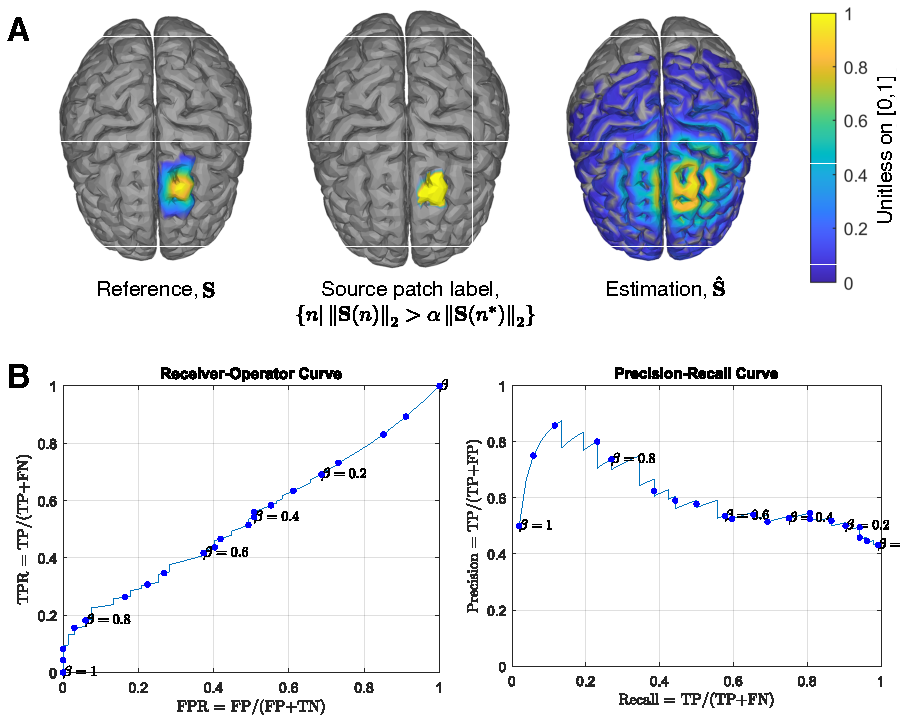
\includegraphics[scale=0.85]{./img/AUROC_sketch.pdf}
%
\caption{
A. The true class labels are defined from the true sources, $\SA$, while the estimated labels are constructed from the ESI estimation, $\hat{\SA}$.
Notice the severe class imbalance between yellow and colorless (gray).
%
B. Construction of Receiver Operator Curve (ROC) and Precision-Recall Curve; the area under them is called AUROC and Average Precision, respectively.
%
C. To alleviate the class imbalance, only the dipoles within a certain distance of the patch center are considered; such distance is set to 25.7 \si{mm} to consider approximately 50\% of dipoles in each category.
\\
%
Data for these graphs was obtained from a single trial of synthetic data described in Chapter \ref{ch:numeric}. Reference source distribution $\SA$ was constructed with no-noise and the source estimate $\hat{\SA}$ was computed using sLORETA
}
\label{fig:AUROC}
\end{figure}

%For ease of notation, the labels must be 0/1 must be read as false/true so that we can use the logical operators and ($\wedge$) and not ($\neg$), but also count the number of \textit{true} elements using the carnality ($\abss{\bullet}$).
%
With this notation, we define True Positives, False Positives, True Negatives, and False Negatives as follows
\begin{align}
\text{TP}(\beta)
&=
\sum_{n=1}^N 
\spar{\mathcal{E}_\beta\ppar{n}}
\spar{\mathcal{R}_\beta\ppar{n}}
\label{eq_auroc:1}
\\
\text{FP}(\beta)
&=
\sum_{n=1}^N 
\spar{1-\mathcal{E}_\beta\ppar{n}}
\spar{\mathcal{R}_\beta\ppar{n}}
\label{eq_auroc:2}
\\
\text{TN}(\beta)
&=
\sum_{n=1}^N 
\spar{1-\mathcal{E}_\beta\ppar{n}}
\spar{1-\mathcal{R}_\beta\ppar{n}}
\label{eq_auroc:3}
\\
\text{FN}(\beta)
&=
\sum_{n=1}^N 
\spar{1-\mathcal{E}_\beta\ppar{n}}
\spar{\mathcal{R}_\beta\ppar{n}}
\label{eq_auroc:4}
\end{align}
%Notice that these quantities change as a function of $\beta$.
\begin{comment}
\begin{align}
\text{TP}(\beta)
&=
\sum_{n=1}^N 
\spar{\mathcal{R}_\beta\ppar{n}}
\spar{\mathcal{E}_\beta\ppar{n}}
\abss{ 
\mathcal{A}_n^{\text{ref}}(\beta) \wedge 
\mathcal{A}_n^{\text{est}}(\beta) }
\\
\text{FP}
&=
\abss{ 
\neg \mathcal{A}_n^{\text{ref}}(\beta) \wedge 
\mathcal{A}_n^{\text{est}}(\beta) }
\\
\text{TN}
&=
\abss{ 
\neg \mathcal{A}_n^{\text{ref}}(\beta) \wedge 
\neg \mathcal{A}_n^{\text{est}}(\beta) }
\\
\text{FN}
&=
\abss{ 
\mathcal{A}_n^{\text{ref}}(\beta) \wedge 
\neg \mathcal{A}_n^{\text{est}}(\beta) }
\end{align}
\end{comment}

The Receiver-Operator Curve (ROC) itself is the parametric curve defined by
$\ppar{\text{FPR}\ppar{\beta}, \text{TPR}\ppar{\beta}}$, where the False Positive Rate (FPR) and True Positive Rate (TPR) are defined as
\begin{align}
\text{FPR}(\beta)
&=
\frac{ \text{FP}\ppar{\beta} }{\text{FP}\ppar{\beta} + \text{TN}\ppar{\beta}}
\\
\text{TPR}(\beta)
&=
\frac{ \text{TP}\ppar{\beta} }{\text{TP}\ppar{\beta} + \text{FN}\ppar{\beta}}
\end{align}

The interpretation of the Receiver-Operator Curve is that each selection of $\beta$ balances the ratios of True Positives and False Negatives:
\begin{itemize}
\item 
Large $\beta$ $\implies$ labels will be strict, with very few False Positives but many False Negatives.
\item
Small $\beta$ $\implies$ labels will be permissive, with very few False Negatives but many False Positives.
\end{itemize}
In general, extreme values of $\beta$ will lead to the endpoints (0,0) and (1,1) of the ROC, and a somewhat smooth trajectory will be observed as $\beta$ increases.

A classifier for which TPR$(\beta)\approx 1$ and FPR$(\beta)\approx 0$ for all $\ beta$'s is preferable whenever possible.
%
Visually, this condition means that the ROC is `close to the top.'

This concept is formalized by taking the area under the ROC (AUROC): the area inside $[0,1]^2\subset \R^2$ below the ROC curve.
%
In practice, the AUROC can be computed numerically using the trapezoid rule as follows
\begin{equation}
\text{AUROC} =
\frac{1}{2}
\sum_{i}
\ppar{ \text{FPR}\ppar{\beta_i}-\text{FPR}\ppar{\beta_{i-1}} }
\ppar{ \text{TPR}\ppar{\beta_i}+\text{TPR}\ppar{\beta_{i-1}} }
\end{equation}
with $\beta_i$ the finite number of values that $\beta$ can take.

%The condition described previously that the ROC must be `close to the top' can be rewritten as 
%AUROC$\approx 1$ being preferable.

With this definition at hand, we can rewrite the most desirable scenario where AUROC $\approx 1$.

\subsubsection{Local AUROC}

AUROC can be biased on the presence of severe class imbalance when a class has many more elements than the other.
%
This phenomenon is represented in figure \ref{fig:AUROC}: panel A shows how the reference labels created using $\beta_0$ only account for a tiny fraction of dipoles available in the model, while panel B shows that the ROC is unusually flat, regardless of the quality of the ESI estimation.

The class imbalance can't be avoided on the ESI since the source patches are globally sparse and compact --or at least we assume that.

One option to alleviate this issue is to consider only a small selection of dipoles for classification.
%
In other words, construct local estimated labels as
\begin{align}
\mathcal{E}_\beta^{(d)}(n)
&=
\begin{cases}
1, &\text{if }
\nnorm{\hat{\SA}(n)}_2 \geq \beta \max_{n'}\sset{\nnorm{\hat{\SA}(n')}_2}
\text{ and }
\nnorm{\rr_n-\mathbf{m}_p}<d
\\
0, &\text{otherwise}
\end{cases}
\end{align}
with $\rr_n$ the location of the $n$-th dipole, $\mathbf{m}_*$ the location of the center of the closest source patch, and $d>0$ a parameter controlling how many dipoles are to be considered.

We can define local target labels analogously.
%
To compute local true/false positives/negatives, we must consider only `local' dipoles.
%
For example, 
%the local True Positive would be defined as
\begin{align}
    \text{TP}^{(d)}(\beta)
&=
\sum_{\substack{n\in \sset{1, \dots, N} \\ \nnorm{\rr_n-\mathbf{m}_p}<d}}
\spar{\mathcal{E}^{(d)}_\beta\ppar{n}}
\spar{\mathcal{R}^{(d)}_\beta\ppar{n}}
\end{align}

This construction leads to a local AUROC.
%
In order to satisfy it's purpose, $d$ must be selected so that
$\frac{1}{N} \sum_{n=1}^N \mathcal{R}^{(d)}_{\beta_0} (n) \approx 0.5$ for a suitable $\beta_0$.

%The suffix `global' is added since all the dipoles are used to compute AUROC.
%
%Some authors proposed that the AUROC value may be imprecise due to the severe class imbalance; we expect the proportion of active dipoles at any moment to be very low.
%
%To alleviate that, they propose to use dipoles within a certain distance from the true center.
%
%We refer to that metric as $\text{AUROC}_\text{local}$ and use the distance as 5 \si{mm}.

\begin{comment}
\begin{figure}
\centering
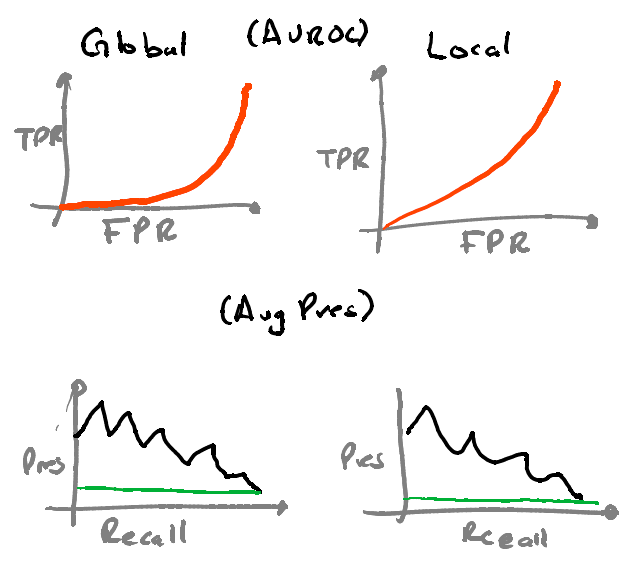
\includegraphics[width=0.8\linewidth]{./img_dev/nsCurves4}
\caption{effect of neighborhood radius over the Receiver-Operator Curve and the Precision-Recall Curve. To attenuate the effects of class imbalance on the active/non-active dipoles, a small neighborhood around the source patch center is considered for the construction of the Receiver-Operator Curve and the Precision-Recall Curve, and in turn to compute the AUROC and Average Precision.
%
Data for these graphs was obtained from a single run of the protocol for synthetic data described in Chapter \ref{ch:numeric}, while the estimates $\SA_\lambda$ were computed using sLORETA}
\end{figure}
\end{comment}

\subsection{Average Precision}

A different approach to class imbalance is using a different quantity with properties similar to AUROC.
%
Average Precision, also known as Area Under Precision-Recall Curve, is based on the parametric curve 
$\ppar{\text{Rec}\ppar{\beta}, \text{Pre}\ppar{\beta}}$, where the Precision (Pre) and Rec (Rec) are defined as
\begin{align}
\text{Pre}\ppar{\beta}
&=
\frac{ \text{TP}\ppar{\beta} }{\text{TP}\ppar{\beta} + \text{FP}\ppar{\beta}}
\\
\text{Rec}\ppar{\beta}
&=
\frac{ \text{TP}\ppar{\beta} }{\text{TP}\ppar{\beta} + \text{FP}\ppar{\beta}}
\end{align}
where the true/false positive/negatives are defined as in equations 
\ref{eq_auroc:1},
\ref{eq_auroc:2},
\ref{eq_auroc:3}, and
\ref{eq_auroc:4}.

Similar to AUROC, Average Precision can be computed numerically as follows
\begin{equation}
\text{Avg. Pre.} =
\frac{1}{2}
\sum_{i}
\ppar{ \text{FPR}\ppar{\beta_i}-\text{FPR}\ppar{\beta_{i-1}} }
\ppar{ \text{TPR}\ppar{\beta_i}+\text{TPR}\ppar{\beta_{i-1}} }
\end{equation}

Average Precision ranges from 0 to 1, with 1 being preferable.

Although the definition of Average Precision is very similar to that of AUROC, it is different in many aspects.
%
For example, the Precision-Recall Curve is somewhat decreasing but displays some sharp zigzags. 
%
When the recall is approximately 1, the precision is roughly equal to the ratio of elements between classes.

Similar to AUROC, defining a `local' Average Precision is possible.
%
In figure \ref{fig:AUROC}, we can observe that the Precision-Recall Curve is quite similar to its global counterpart, or at least when compared against the local and global ROC.
%
Informally, we may observe that Average Precision is more robust to the class imbalance.